\documentclass[12pt,letterpaper]{article}

% ---------- Paquetes ----------
\usepackage[utf8]{inputenc}
\usepackage[T1]{fontenc}
\usepackage[spanish]{babel}
\usepackage[margin=3cm]{geometry}
\usepackage{graphicx}
\usepackage{enumitem}
\usepackage{hyperref}
\usepackage{xurl}
\usepackage{titlesec}
\usepackage{parskip}
\usepackage{array}

\hypersetup{
    colorlinks=true,
    linkcolor=black,
    urlcolor=blue,
    citecolor=black
}

\titleformat{\section}{\large\bfseries}{\thesection.}{0.5em}{}
\titleformat{\subsection}{\normalsize\bfseries}{\thesubsection}{0.5em}{}

\setlength{\parindent}{0pt}
\setlength{\parskip}{6pt}

\begin{document}

% ==================================================
% PORTADA
% ==================================================
\begin{titlepage}
    \centering
    \vspace*{1cm}

    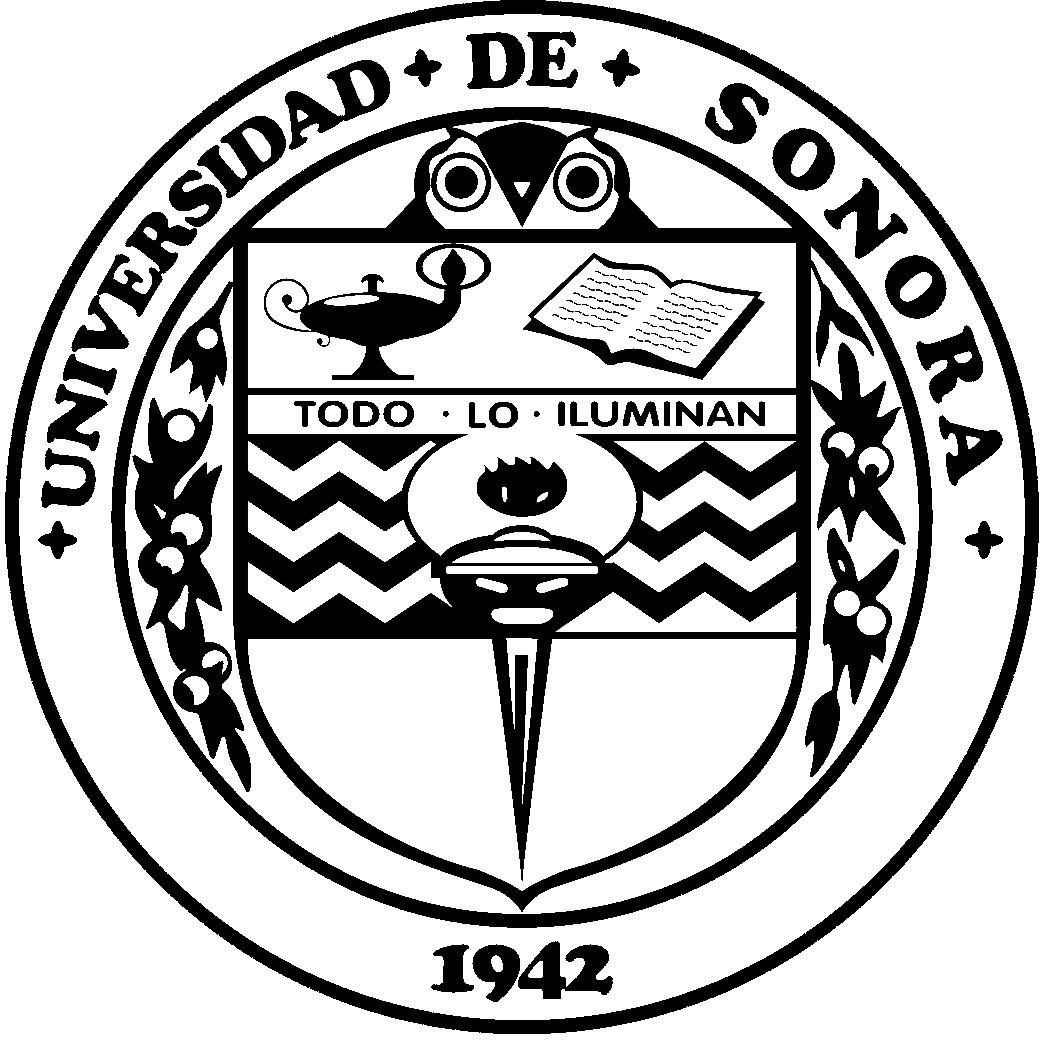
\includegraphics[width=4cm]{escudo.png}

    \vspace{0.5cm}

    {\Large \textbf{Universidad de Sonora}}\\[0.3cm]
    {\large Licenciatura en Ciencias de la Computación}

    \vspace{1.8cm}

    {\Large \textbf{Investigación sobre la Red de Satélites Starlink}}\\[0.3cm]
    {\large Investigación documental y reporte}

    \vspace{1.8cm}

    \begin{tabular}{rl}
        \textbf{Materia:} & Redes de Computadoras I \\[4pt]
        \textbf{Periodo:} & 2026-2 \\[4pt]
        \textbf{Profesor:} & Dr. Donald José Rodríguez Úbeda \\
    \end{tabular}

    \vspace{1.3cm}

    {\large \textbf{Integrantes del equipo}}

    \vspace{0.4cm}

    \begin{tabular}{ll}
        Angel Alberto Amaya Soria & Expediente 223210350 \\[4pt]
        Angel Fernando Bórquez Guerrero & Expediente 219208106 \\[4pt]
        Emily Margarita Beltrán Zazueta & Expediente 223203546 \\[4pt]
        Gabriela Aydee Miranda & Expediente 222220740 \\[4pt]
        Javier Leonardo Miranda Sánchez & Expediente 223215039 \\
    \end{tabular}

    \vfill

    {\large Hermosillo, Sonora \hspace{1cm} Octubre de 2026}

\end{titlepage}

% ==================================================
% ÍNDICE
% ==================================================
\tableofcontents
\newpage

% ==================================================
% CONTENIDO
% ==================================================
\section{Introducción}

Starlink es la red de internet satelital de la empresa SpaceX y, por el número de satélites en operación, es hoy la constelación más grande jamás desplegada. Este reporte responde las nueve preguntas planteadas en la tarea: qué es y cuál es su objetivo, cuántos satélites tiene y en qué órbita se encuentran, cuántos se planea instalar, qué bandas y frecuencias utiliza, qué latencia ofrece, qué factores afectan sus transmisiones, cuál es su cobertura, por qué no es global y cuáles son las especificaciones físicas de sus satélites. Las cifras de una constelación en crecimiento cambian casi a diario, por lo que, salvo que se indique otra cosa, los datos corresponden a octubre de 2026.

\section{¿En qué consiste la red Starlink y cuál es su objetivo?}

Starlink es una constelación de satélites de internet que opera en órbita terrestre baja (LEO) y que proporciona acceso a internet de banda ancha a gran parte del planeta (Wikipedia, 2026a). Se compone de tres segmentos:

\begin{itemize}[nosep]
    \item \textbf{Segmento espacial:} los satélites, que reciben el tráfico de los usuarios y lo envían a estaciones en tierra. Desde la generación v1.5, los satélites incluyen enlaces láser entre sí, de modo que pueden pasarse los datos en el espacio sin depender siempre de una estación terrena (SatFleet Live, 2026).
    \item \textbf{Segmento terrestre:} estaciones o \textit{gateways} conectadas a la red troncal de internet, que sirven de puente entre los satélites y la red terrestre (CellStream, 2026).
    \item \textbf{Segmento de usuario:} el terminal del cliente, una antena de arreglo en fase (\textit{phased array}) que apunta electrónicamente, sin partes móviles, al satélite que tiene a la vista, junto con un enrutador Wi-Fi (CellStream, 2026).
\end{itemize}

El \textbf{objetivo} de Starlink es ofrecer internet de alta velocidad y baja latencia a nivel mundial, especialmente en zonas rurales o remotas donde la infraestructura terrestre (fibra, cable o torres) es limitada o inexistente, así como en barcos, aviones y vehículos en movimiento. La Federal Communications Commission (FCC, 2026a), al autorizar la segunda generación del sistema, describe esa meta como la entrega de servicio de banda ancha de alta velocidad y baja latencia a escala global, incluyendo servicio móvil y cobertura complementaria desde el espacio. Además de su servicio principal, SpaceX ha desarrollado satélites con conexión directa a teléfonos celulares (\textit{Direct to Cell}), usados con operadores aliados como T-Mobile (SatFleet Live, 2026). SpaceX informó en junio de 2026 que Starlink contaba con más de 12 millones de clientes activos en más de 160 países y territorios (SatFleet Live, 2026).

\section{Satélites instalados actualmente, órbita y distancia a la Tierra}

\subsection{Número de satélites}

Existen tres cifras que conviene distinguir: los satélites lanzados en total, los que siguen en órbita y los que funcionan. Según el astrónomo Jonathan McDowell, quien registra individualmente cada satélite, al 2 de octubre de 2026 se habían lanzado 12,988 satélites Starlink, de los cuales 11,156 seguían en órbita y 11,142 estaban funcionando; unos 9,727 ya se encontraban en sus órbitas operativas finales, 235 estaban elevando su órbita tras el lanzamiento y 151 estaban siendo retirados, mientras que 1,832 ya habían reingresado a la atmósfera (SatFleet Live, 2026). Otro rastreador reporta 11,166 satélites en órbita y 11,151 funcionando al 26 de octubre de 2026 (KeepTrack, 2026a). Las diferencias entre fuentes se deben a la fecha de corte y a qué se considera un satélite ``activo''; en términos generales, \textbf{Starlink tiene alrededor de 11,100 satélites en órbita}, lo que equivale a cerca de dos tercios de todos los satélites activos del mundo (SatFleet Live, 2026; azmth, 2026).

\subsection{Órbita y altitud}

Los satélites Starlink se encuentran en \textbf{órbita terrestre baja (LEO)}, organizados en \textit{shells} o capas: conjuntos de órbitas con una altitud e inclinación similares. La inclinación determina qué tan al norte y al sur llega cada capa. A continuación se muestra la distribución de los satélites activos por inclinación al 7 de octubre de 2026 (SatFleet Live, 2026):

\begin{center}
\begin{tabular}{|c|c|c|}
\hline
\textbf{Inclinación de la capa} & \textbf{Satélites activos} & \textbf{Porcentaje} \\
\hline
53° & 5,102 & 45.8\,\% \\
\hline
43° & 3,615 & 32.5\,\% \\
\hline
70° & 870 & 7.8\,\% \\
\hline
Polar (97°) & 1,526 & 13.7\,\% \\
\hline
Otras & 26 & 0.2\,\% \\
\hline
\end{tabular}
\end{center}

En cuanto a la \textbf{distancia a la Tierra}, el satélite típico orbita a unos 466~km de altura, y cerca del 87\,\% de los satélites activos vuela entre 400 y 520~km (SatFleet Live, 2026). Originalmente la mayoría de los satélites operaba a unos 550~km; sin embargo, en enero de 2026 SpaceX anunció que bajaría a unos 480~km los cerca de 4,400 satélites de esa altitud a lo largo del año, con el fin de mejorar la seguridad espacial, ya que a menor altura hay menos desechos y un satélite averiado cae más rápido (CNBC, 2026; SatFleet Live, 2026). Además, la FCC autorizó nuevas capas de entre 340 y 485~km (FCC, 2026a). Para dar una idea de escala, esta altura es unas 75 veces menor que la de un satélite geoestacionario (cerca de 35,800~km) (SatFleet Live, 2026). A 480~km, un satélite viaja a unos 27,400~km/h y completa una vuelta a la Tierra en aproximadamente 94 minutos, es decir, más de 15 vueltas al día (SatFleet Live, 2026).

\section{Satélites proyectados}

La cantidad de satélites que se planea instalar depende de las autorizaciones regulatorias:

\begin{itemize}[nosep]
    \item \textbf{Primera generación:} la FCC autorizó alrededor de 4,400 satélites (SatFleet Live, 2026).
    \item \textbf{Segunda generación (Gen2):} el 9 de enero de 2026 la FCC aprobó 7,500 satélites adicionales, con lo que el total autorizado de esta generación asciende a \textbf{15,000}; los 14,988 restantes que SpaceX había solicitado quedaron diferidos para una decisión posterior (FCC, 2026a; Total Telecom, 2026). Como condición, SpaceX debe tener en operación el 50\,\% de los nuevos satélites a más tardar el 1 de diciembre de 2028 y el resto para el 1 de diciembre de 2031 (Tom's Hardware, 2026).
    \item \textbf{Conexión directa a dispositivos:} el 6 de octubre de 2026 la FCC concedió parcialmente un sistema de 15,000 satélites en capas a 326--335~km, con la mitad en operación para octubre de 2032 y el resto para octubre de 2035 (azmth, 2026).
    \item \textbf{Solicitudes de SpaceX:} la empresa pidió cerca de 30,000 satélites de segunda generación. La cifra de 42,000 que suele citarse proviene de planes anteriores que sumaban unos 12,000 satélites de primera generación a esos 30,000, y es un total solicitado en algún momento, no lo que está autorizado hoy (SatFleet Live, 2026).
\end{itemize}

En resumen, lo autorizado por la FCC es del orden de 19,400 satélites de las dos primeras generaciones (a los que se suman los de conexión directa a dispositivos), y SpaceX aspira a una cifra considerablemente mayor.

\section{Banda y frecuencias de operación}

Starlink emplea distintas bandas según el tipo de enlace, resumidas en la siguiente tabla:

\begin{center}
\small
\begin{tabular}{|>{\raggedright\arraybackslash}p{3.4cm}|>{\raggedright\arraybackslash}p{4.1cm}|>{\raggedright\arraybackslash}p{1.5cm}|>{\raggedright\arraybackslash}p{4.8cm}|}
\hline
\textbf{Enlace} & \textbf{Sentido} & \textbf{Banda} & \textbf{Frecuencias} \\
\hline
Usuario (descarga) & Satélite $\rightarrow$ terminal & Ku & 10.7--12.7 GHz \\
\hline
Usuario (subida) & Terminal $\rightarrow$ satélite & Ku & 14.0--14.5 GHz \\
\hline
Gateway (bajada) & Satélite $\rightarrow$ gateway & Ka & 17.8--18.6 GHz y 18.8--19.3 GHz \\
\hline
Gateway (subida) & Gateway $\rightarrow$ satélite & Ka & 27.5--29.1 GHz y 29.5--30.0 GHz \\
\hline
Gateway de alta capacidad (bajada) & Satélite $\rightarrow$ gateway & E & 71--76 GHz \\
\hline
Gateway de alta capacidad (subida) & Gateway $\rightarrow$ satélite & E & 81--86 GHz \\
\hline
\end{tabular}
\end{center}

Fuentes: CellStream (2026) y KeepTrack (2026b).

Los terminales de usuario se comunican con los satélites en la \textbf{banda Ku}: reciben en el rango de 10.7 a 12.7~GHz (aproximadamente 2~GHz de ancho de banda dividido en canales de 250~MHz) y transmiten en 14.0 a 14.5~GHz (500~MHz) (CellStream, 2026; KeepTrack, 2026b). Los satélites se enlazan con las estaciones terrenas principalmente en la \textbf{banda Ka}, y las estaciones más recientes y de mayor capacidad también usan la \textbf{banda E} (CellStream, 2026). Entre los propios satélites, la comunicación se realiza mediante enlaces ópticos (láser) (SatFleet Live, 2026).

Adicionalmente, la autorización de la FCC para la segunda generación permite operar en otras bandas, entre ellas Ku, Ka, V, E y W, para servicio fijo y móvil por satélite (FCC, 2026b), así como en el rango de 1,429 a 2,690~MHz para el servicio de conexión directa a teléfonos celulares fuera de Estados Unidos (FCC, 2026b).

\section{Latencia de las transmisiones}

La latencia es el tiempo que tarda un dato en ir y volver entre el usuario y el servidor. En Starlink depende, en primer lugar, de la distancia: una señal que viaja a unos 550~km tarda alrededor de 1.8~ms en llegar al satélite, y el tiempo total de ida y vuelta, que incluye el procesamiento y el trayecto hasta la estación terrena, ronda entre 25 y 50~ms (Orbital Radar, 2026). En contraste, los servicios satelitales de órbita geoestacionaria tienen típicamente 600~ms o más, porque el satélite se encuentra a decenas de miles de kilómetros (US Mobile, 2026).

Las mediciones independientes de Ookla en Estados Unidos reportan latencias medianas cercanas a 38--39~ms en los estados con mejor desempeño (Washington D.~C., Arizona, Colorado y Nueva Jersey), mientras que en Alaska y Hawái alcanzan 105 y 115~ms, respectivamente; SpaceX tiene como meta una latencia mediana de 20~ms (Macfarlane, 2026). En el uso cotidiano, la mayoría de los usuarios observa entre 25 y 50~ms, con medianas de alrededor de 31 a 35~ms hacia finales de 2025 (US Mobile, 2026). Según Ookla, la latencia ha mejorado a nivel mundial en los principales mercados de Starlink (Via Satellite, 2026).

La latencia aumenta cuando la red está saturada, cuando el terminal está lejos de una estación terrena o cuando el tráfico debe viajar más tiempo por la constelación antes de bajar a tierra.

\section{Afectaciones que pueden sufrir las transmisiones}

\begin{itemize}[nosep]
    \item \textbf{Lluvia, nieve y tormentas (\textit{rain fade}):} las frecuencias altas son absorbidas y dispersadas por las gotas de agua, por lo que la lluvia intensa o la nieve pueden causar reducciones de velocidad o interrupciones breves, que normalmente se restablecen en minutos cuando pasa lo más fuerte de la tormenta; la lluvia ligera casi no afecta el servicio (DishyCentral, 2026b).
    \item \textbf{Obstrucciones físicas:} árboles, edificios u otros objetos que bloquean la vista del cielo hacen que el terminal pierda al satélite durante los cambios de uno a otro, provocando microcortes (DishyCentral, 2026b).
    \item \textbf{Congestión de la red:} en zonas con muchos suscriptores, las velocidades pueden bajar y la latencia subir durante las horas pico, y algunos planes tienen menor prioridad ante saturación (DishyCentral, 2026a; Pong, 2026).
    \item \textbf{Fallas en tierra y de software:} las interrupciones de las estaciones terrenas o de su conexión troncal y las actualizaciones de software pueden dejar sin servicio a muchos usuarios; por ejemplo, en julio de 2025 ocurrió una caída global de casi tres horas por una actualización del firmware de las estaciones (Zlatev, 2025).
    \item \textbf{Clima espacial:} las tormentas geomagnéticas aumentan la resistencia del aire en la atmósfera superior; en febrero de 2022 una tormenta considerada menor provocó la pérdida de 38 de 49 satélites recién lanzados (Cooperative Institute for Research in Environmental Sciences, s.f.), y en mayo de 2024 una tormenta extrema degradó el servicio, aunque la constelación siguió operando (Wikipedia, 2026b). Otra caída global de septiembre de 2025 coincidió con una alerta de tormenta geomagnética (Zlatev, 2025).
    \item \textbf{Restricciones regulatorias:} en los países donde Starlink no tiene autorización, el servicio está bloqueado geográficamente, aunque se tenga el equipo (Starlink News, 2026).
\end{itemize}

\section{Cobertura, calidad del servicio y países con acceso}

\subsection{¿Tiene cobertura global?}

Físicamente, la constelación rodea todo el planeta, pero Starlink solo ofrece servicio en los países donde cuenta con licencia del gobierno y autorización para usar el espectro (Starlink Info, 2026). Por lo tanto, \textbf{no tiene cobertura global} en sentido comercial.

\subsection{¿La tasa de transferencia y la calidad del servicio son las mismas en todo el planeta?}

No. El desempeño varía según la densidad de suscriptores, la cercanía de estaciones terrenas y el tiempo que lleva operando el servicio en cada lugar (Earthsims, 2026). Según Ookla, entre los países con mayores medianas de descarga se encuentran Letonia, las Islas Marianas del Norte, Nueva Zelanda, Azerbaiyán y Portugal, con más de 180~Mbps, mientras que Sudán del Sur, Madagascar y Liberia registran entre 16 y 27~Mbps (Via Satellite, 2026). En Estados Unidos, la mediana de descarga pasó de 53.95~Mbps en el tercer trimestre de 2022 a 104.71~Mbps en el primero de 2025, y la latencia también varía entre estados (Macfarlane, 2026). Las velocidades medidas por Ookla tampoco coinciden con las anunciadas por SpaceX, que reporta medianas superiores a 200~Mbps en 2025 (Via Satellite, 2026).

\subsection{¿En qué países o regiones se puede acceder al servicio?}

Según el mapa de disponibilidad de Starlink (actualizado el 22 de septiembre de 2026), el servicio está disponible en \textbf{172 países y territorios}; otros 58 están marcados como ``próximamente'' y 6 esperan aprobación regulatoria (Brunéi, India, Pakistán, Arabia Saudita, Tailandia y Turquía) (DishyCentral, 2026a). Abarca la mayor parte de América, Europa, África subsahariana y Oceanía (Mappr, 2026). Entre los mercados más grandes por volumen de mediciones de Ookla se encuentran Estados Unidos, México, Indonesia, Brasil y Canadá (Via Satellite, 2026), por lo que México es uno de los principales mercados de Starlink.

\section{Razones por las que no existe cobertura global}

\begin{itemize}[nosep]
    \item \textbf{Países donde está prohibido o no se ofrece:} el mapa de Starlink marca ocho territorios sin servicio: Afganistán, Bielorrusia, China, Hong Kong, Macao, Corea del Norte, Rusia y Siria (DishyCentral, 2026a). En varios de ellos (China, Rusia, Irán y Corea del Norte) no existe una autorización comercial, ya que las leyes de seguridad nacional, ciberseguridad o las sanciones excluyen a operadores extranjeros (Starlink News, 2026).
    \item \textbf{Licencias y espectro:} cada país debe autorizar la operación y el uso de las frecuencias; mientras el regulador no lo apruebe, Starlink no puede vender servicio, como ocurre en India o Pakistán (DishyCentral, 2026a).
    \item \textbf{Control gubernamental de las telecomunicaciones:} en algunos países, el Estado mantiene un control estricto del acceso a internet, lo que impide el uso legal de un sistema que no depende de su infraestructura (Starlink News, 2026).
    \item \textbf{Capacidad e infraestructura:} el servicio depende de las estaciones terrenas y de la capacidad disponible en cada zona; donde hay pocas estaciones o muchos usuarios, la calidad es menor (DishyCentral, 2026a; Earthsims, 2026).
    \item \textbf{Geometría orbital:} la mayoría de los satélites está en capas de 43° y 53°, que cubren sobre todo las latitudes donde vive la mayor parte de la población; las regiones polares dependen de las capas de 70° y 97° (SatFleet Live, 2026).
\end{itemize}

\section{Especificaciones físicas de los satélites}

El diseño de los satélites ha cambiado con cada generación, siendo cada vez más grandes y con más capacidad:

\begin{center}
\small
\begin{tabular}{|>{\raggedright\arraybackslash}p{2.3cm}|>{\raggedright\arraybackslash}p{2.4cm}|>{\raggedright\arraybackslash}p{2.1cm}|>{\raggedright\arraybackslash}p{7.0cm}|}
\hline
\textbf{Generación} & \textbf{Masa} & \textbf{Lanzados$^*$} & \textbf{Características} \\
\hline
v1.0 & 260 kg & 1,665 & Cuerpo plano con un solo panel solar; antenas de banda Ku y Ka; sin enlaces láser (SatFleet Live, 2026; Wikipedia, 2026a). \\
\hline
v1.5 & 295--306 kg & 2,987 & Primera con enlaces láser entre satélites (SatFleet Live, 2026; Wikipedia, 2026a). \\
\hline
V2 Mini & aprox.\ 740--800 kg & 8,282 & Cuerpo de 4.1 $\times$ 2.7 m; dos paneles solares de 4.1 $\times$ 12.8 m cada uno (envergadura de unos 30 m); superficie total de unos 116 m$^2$; cuatro veces la capacidad de una v1.5; antenas de arreglo en fase mayores y banda E; propulsión eléctrica con propelente de argón (McDowell, s.f.; Spaceflight Now, 2023; Wikipedia, 2026a). \\
\hline
V2 & aprox.\ 1,250 kg & 38 & Versión de mayor tamaño, pensada para lanzarse con Starship (Wikipedia, 2026a). \\
\hline
V3 & no publicada$^{**}$ & 46 (26 en órbita) & Diseñada para Starship; según SpaceX, con más de diez veces la capacidad de una V2 (SatFleet Live, 2026; azmth, 2026). \\
\hline
\end{tabular}
\end{center}

{\footnotesize $^*$Según la lista de lanzamientos de Wikipedia al 23 de octubre de 2026 (Wikipedia, 2026a); los de V3 incluyen 20 satélites lanzados en una trayectoria suborbital en julio de 2026 (azmth, 2026). $^{**}$Las fuentes consultadas no reportan la masa de la V3.}

Otras características comunes de los satélites son:

\begin{itemize}[nosep]
    \item \textbf{Propulsión:} usan motores eléctricos de efecto Hall para maniobrar en órbita. Los primeros emplean kriptón y los V2 Mini, argón, que es más barato; este último sistema ofrece 2.4 veces el empuje y 1.5 veces el impulso específico del anterior (Newspace.im, s.f.; Spaceflight Now, 2023).
    \item \textbf{Comunicaciones:} antenas de arreglo en fase para los enlaces con usuarios (Ku) y estaciones terrenas (Ka y E), y enlaces láser entre satélites (SatFleet Live, 2026; Wikipedia, 2026a).
    \item \textbf{Vida útil y retiro:} están diseñados para durar unos cinco años; al final, SpaceX baja su órbita con los propulsores hasta que se desintegran en la atmósfera (SatFleet Live, 2026).
    \item \textbf{Brillo:} para reducir su impacto en la astronomía, los satélites lanzados desde mediados de 2020 llevaron un parasol (VisorSat), que se eliminó en la v1.5 porque bloqueaba los láseres; los V2 Mini usan una película de espejo dieléctrico (SatFleet Live, 2026; TrackStarlink, 2026).
\end{itemize}

\section{Conclusión}

Starlink es una constelación de más de 11,000 satélites en órbita baja, entre 340 y 550~km de altura, que combina enlaces de radio en las bandas Ku, Ka y E, enlaces láser entre satélites y terminales de usuario de arreglo en fase para ofrecer internet de baja latencia, típicamente entre 25 y 50~ms. Su crecimiento continúa, con decenas de miles de satélites autorizados o solicitados y la llegada de la generación V3. Sin embargo, su servicio no es verdaderamente global ni uniforme: depende de licencias gubernamentales, de la geopolítica, de la infraestructura terrestre y de la saturación de la red, además de verse afectado por el clima, las obstrucciones y la actividad solar.

% ==================================================
% REFERENCIAS (formato APA)
% ==================================================
\newpage
\section*{Referencias}
\addcontentsline{toc}{section}{Referencias}

\begin{itemize}[leftmargin=1.5em,itemsep=7pt]

\item[] azmth. (2026, 9 de octubre). \textit{Starlink tracker: Live Starlink satellite map in 3D}. \url{https://azmth.space/tracker/starlink}

\item[] CellStream, Inc. (2026, 29 de junio). \textit{What is the Starlink operational model?} \url{https://www.cellstream.com/2026/06/29/what-is-the-starlink-operational-model/}

\item[] Cooperative Institute for Research in Environmental Sciences. (s.f.). \textit{Minor geomagnetic storm, big impact: The February 2022 Starlink satellite loss}. University of Colorado Boulder. \url{https://cires.colorado.edu/news/minor-geomagnetic-storm-big-impact-february-2022-starlink-satellite-loss}

\item[] CNBC. (2026, 10 de enero). \textit{FCC approves SpaceX plan to deploy an additional 7,500 Starlink satellites}. \url{https://www.cnbc.com/2026/01/10/fcc-approves-spacex-plan-to-deploy-7500-starlink-satellites.html}

\item[] DishyCentral. (2026a, 22 de septiembre). \textit{Starlink availability map 2026: Every country, updated daily}. \url{https://dishycentral.com/starlink-availability-map}

\item[] DishyCentral. (2026b). \textit{Does Starlink work in bad weather?} \url{https://dishycentral.com/does-starlink-work-in-bad-weather}

\item[] Earthsims. (2026). \textit{Best countries for Starlink 2026: Speed \& availability map}. \url{https://www.earthsims.com/starlink/best-countries-starlink/}

\item[] Federal Communications Commission. (2026a, 9 de enero). \textit{FCC approves next-gen satellite constellation: Enabling better, faster broadband throughout America} [Comunicado de prensa]. \url{https://docs.fcc.gov/public/attachments/DOC-417881A1.pdf}

\item[] Federal Communications Commission, Space Bureau. (2026b). \textit{Orden DA 26-36: SpaceX second-generation Starlink constellation (Gen2 Starlink)}. \url{https://docs.fcc.gov/public/attachments/DA-26-36A1.pdf}

\item[] KeepTrack. (2026a, 26 de octubre). \textit{How many Starlink satellites are in orbit?} \url{https://keeptrack.space/starlink-satellite-count}

\item[] KeepTrack. (2026b). \textit{What is Ku-band? The 12 to 18 GHz band}. \url{https://keeptrack.space/space-terms/ku-band}

\item[] Macfarlane, M. (2026). \textit{Starlink expands subscribers and speeds}. Broadband Breakfast. \url{https://broadbandbreakfast.com/starlink-expands-subscribers-and-speeds/}

\item[] Mappr. (2026, mayo). \textit{Mapped: Where Starlink is available around the world}. \url{https://www.mappr.co/starlink-availability-by-country/}

\item[] McDowell, J. C. (s.f.). \textit{Starlink}. \url{https://planet4589.org/astro/starsim/index.html}

\item[] Newspace.im. (s.f.). \textit{SpaceX (Starlink V2 Mini) --- Satellite constellation}. \url{https://www.newspace.im/constellations/spacex-starlink-v2-mini}

\item[] Orbital Radar. (2026). \textit{Satellite internet speeds \& latency compared}. \url{https://orbitalradar.com/satellite-internet/speeds-and-latency}

\item[] Pong. (2026). \textit{Starlink internet speed: How fast is it really in 2026?} \url{https://www.pong.com/blog/starlink-internet-speed-real-world-test}

\item[] SatFleet Live. (2026, 7 de octubre). \textit{How many Starlink satellites are in orbit right now? Live count}. \url{https://satfleetlive.com/blogs/starlink-satellites/}

\item[] Spaceflight Now. (2023, 26 de febrero). \textit{SpaceX unveils first batch of larger upgraded Starlink satellites}. \url{https://spaceflightnow.com/2023/02/26/spacex-unveils-first-batch-of-larger-upgraded-starlink-satellites/}

\item[] Starlink Info. (2026). \textit{Starlink global coverage: Constellation map, active countries, and real-world limits}. \url{https://www.starlinkinfo.com/starlink-revolutionizing-internet-access-across-the-globe}

\item[] Starlink News. (2026, 19 de septiembre). \textit{Starlink country approvals 2026: Licences, bans, prices}. \url{https://starlink-news.com/2026/09/19/starlink-country-approvals-2026-licences-bans-prices/}

\item[] Tom's Hardware. (2026, 11 de enero). \textit{FCC approves 7,500 additional Starlink Gen2 satellites}. \url{https://www.tomshardware.com/tech-industry/fcc-approves-7500-additional-starlink-gen2-satellites}

\item[] Total Telecom. (2026). \textit{Starlink gets FCC clearance for 7,500 Gen2 satellites}. \url{https://totaltele.com/starlink-gets-fcc-clearance-for-7500-gen2-satellites/}

\item[] TrackStarlink. (2026). \textit{Starlink satellite versions explained: v0.9 to V3}. \url{https://www.trackstarlink.com/guides/starlink-satellite-versions-explained}

\item[] US Mobile. (2026). \textit{How fast is Starlink internet? Speed tests, real data \& what to expect in 2026}. \url{https://www.usmobile.com/blog/starlink-speed/}

\item[] Via Satellite. (2026, 6 de febrero). \textit{Data shows Starlink dominates consumer internet market, at least for now, Ookla analyst says}. \url{https://www.satellitetoday.com/connectivity/2026/02/06/data-shows-starlink-dominates-consumer-internet-market-at-least-for-now-ookla-analyst-says/}

\item[] Wikipedia. (2026a). \textit{List of Starlink and Starshield launches}. En \textit{Wikipedia, the free encyclopedia}. \url{https://en.wikipedia.org/wiki/List_of_Starlink_and_Starshield_launches}

\item[] Wikipedia. (2026b). \textit{May 2024 solar storms}. En \textit{Wikipedia, the free encyclopedia}. \url{https://en.wikipedia.org/wiki/May_2024_solar_storms}

\item[] Zlatev, D. (2025, 15 de septiembre). \textit{Starlink global outage happens again with satellite Internet service down during geomagnetic storm}. Notebookcheck. \url{https://www.notebookcheck.net/Starlink-global-outage-happens-again-with-satellite-Internet-service-down-during-geomagnetic-storm.1114762.0.html}

\end{itemize}

\end{document}
